%%\documentclass[a4paper,12pt,oneside]{llncs}
\documentclass{book}
%\usepackage[right=2cm,left=3cm,top=2cm,bottom=2cm,headsep=0cm]{geometry}

%%%%%%%%%%%%%%%%%%%%%%%%%%%%%%%%%%%%%%%%%%%%%%%%%%%%%%%%%%%
%% Juego de caracteres usado en el archivo fuente: UTF-8
\usepackage{ucs}
\usepackage[utf8x]{inputenc}
\usepackage{eurosym}

%%%%%%%%%%%%%%%%%%%%%%%%%%%%%%%%%%%%%%%%%%%%%%%%%%%%%%%%%%%
%% Juego de caracteres usado en la salida dvi
%% Otra posibilidad: \usepackage{t1enc}
\usepackage[T1]{fontenc}

%%%%%%%%%%%%%%%%%%%%%%%%%%%%%%%%%%%%%%%%%%%%%%%%%%%%%%%%%%%
%% Ajusta maergenes para a4
\usepackage{a4wide}

%%%%%%%%%%%%%%%%%%%%%%%%%%%%%%%%%%%%%%%%%%%%%%%%%%%%%%%%%%%
%% Uso fuente postscript times, para que los ps y pdf queden y pequeños...
\usepackage{times}

%%%%%%%%%%%%%%%%%%%%%%%%%%%%%%%%%%%%%%%%%%%%%%%%%%%%%%%%%%%
%% Posibilidad de hipertexto (especialmente en pdf)
\usepackage{hyperref}

%%%%%%%%%%%%%%%%%%%%%%%%%%%%%%%%%%%%%%%%%%%%%%%%%%%%%%%%%%%
%% Graficos 
\usepackage{graphics,graphicx}

%%%%%%%%%%%%%%%%%%%%%%%%%%%%%%%%%%%%%%%%%%%%%%%%%%%%%%%%%%%
%% Ciertos caracteres "raros"...
\usepackage{latexsym}

%%%%%%%%%%%%%%%%%%%%%%%%%%%%%%%%%%%%%%%%%%%%%%%%%%%%%%%%%%%
%% Matematicas aun más fuertes (american math dociety)
\usepackage{amsmath}

%%%%%%%%%%%%%%%%%%%%%%%%%%%%%%%%%%%%%%%%%%%%%%%%%%%%%%%%%%%
\usepackage{multirow} % para las tablas
\usepackage[spanish,es-tabla]{babel}

%%%%%%%%%%%%%%%%%%%%%%%%%%%%%%%%%%%%%%%%%%%%%%%%%%%%%%%%%%%
%% Fuentes matematicas lo mas compatibles posibles con postscript (times)
%% (Esto no funciona para todos los simbolos pero reduce mucho el tamaño del
%% pdf si hay muchas matamaticas....
\usepackage{mathptm}

%%% VARIOS:
\usepackage{slashbox}
\usepackage{verbatim}
\usepackage{array}
\usepackage{listings}
\usepackage{multirow}
\usepackage{hhline}

%% MARCA DE AGUA
%% Este package de "draft copy" NO funciona con pdflatex
%%\usepackage{draftcopy}
%% Este package de "draft copy" SI funciona con pdflatex
%%%\usepackage{pdfdraftcopy}
%%%%%%%%%%%%%%%%%%%%%%%%%%%%%%%%%%%%%%%%%%%%%%%%%%%%%%%%%%%
%% Indenteacion en español...
\usepackage[spanish]{babel}
\usepackage{Estilos/Apuntes}
\usepackage[svgnames,x11names,table]{xcolor}
\usepackage{listings}
% Para escribir código en C
% \begin{verbatim}[language=C]
% #include <stdio.h>
% int main(int argc, char* argv[]) {
% puts("Hola mundo!");
% }
% \end{verbatim}

\title{{\Huge Altavoz Bluetooth}\\\textcolor{White}{ }\\
	\begin{LARGE} 
		Tarjeta LPC4078FBD80\\
		\textcolor{White}{ }\\
		Diseño Basado en Microprocesadores
	\end{LARGE}
	}
\author{Juan Pedro Rodríguez Gracia\\Jesús Rodríguez Heras}

%%Configuracion del paquete listings
\lstset{language=bash, numbers=left, numberstyle=\tiny, numbersep=10pt, firstnumber=1, stepnumber=1}

\begin{document}
	\maketitle
	\thispagestyle{empty}
	\newpage
	
	\tableofcontents
	\newpage
	
\chapter{Introducción}
\section{Objetivos}
El objetivo principal del proyecto es conseguir un altavoz que reproduzca una canción recibida en tiempo real por una conexión serie establecida mediante una antena bluetooth.

Además, tendremos la opción de truncar las muestras recibidas en tiempo real, siendo capaces de quitar hasta los 16 bits de resolución\footnote{Una canción recibida estaría compuesta por dos muestras de 16 bits, una para el altavoz izquierdo y otra para el derecho.}.
\section{Metas}
La meta del proyecto es ser capaces de controlar la cantidad de bits de una canción recibida por bluetooth que llegará a los altavoces con una una resolución menor o igual a 16 bits.

\chapter{Hardware empleado}
El hardware empleado en este proyecto ha sido el siguiente:
\begin{itemize}
	\item Tarjeta LPC4078FBD80.
	\item Codec de audio UDA1380.
	\item Antena bluetooth CZ-HC-05.
	\item Pantalla LCD 16x2.
	\item Amplificador de audio.
\end{itemize}

Todo ello con el software necesario para el control del codec de audio y de la pantalla LCD.
\newpage
\section{Cableado del hardware}
En la siguiente imagen podemos ver el cableado de los pines de los componentes hardware hacia los pines del procesador de la placa.
\begin{center}
	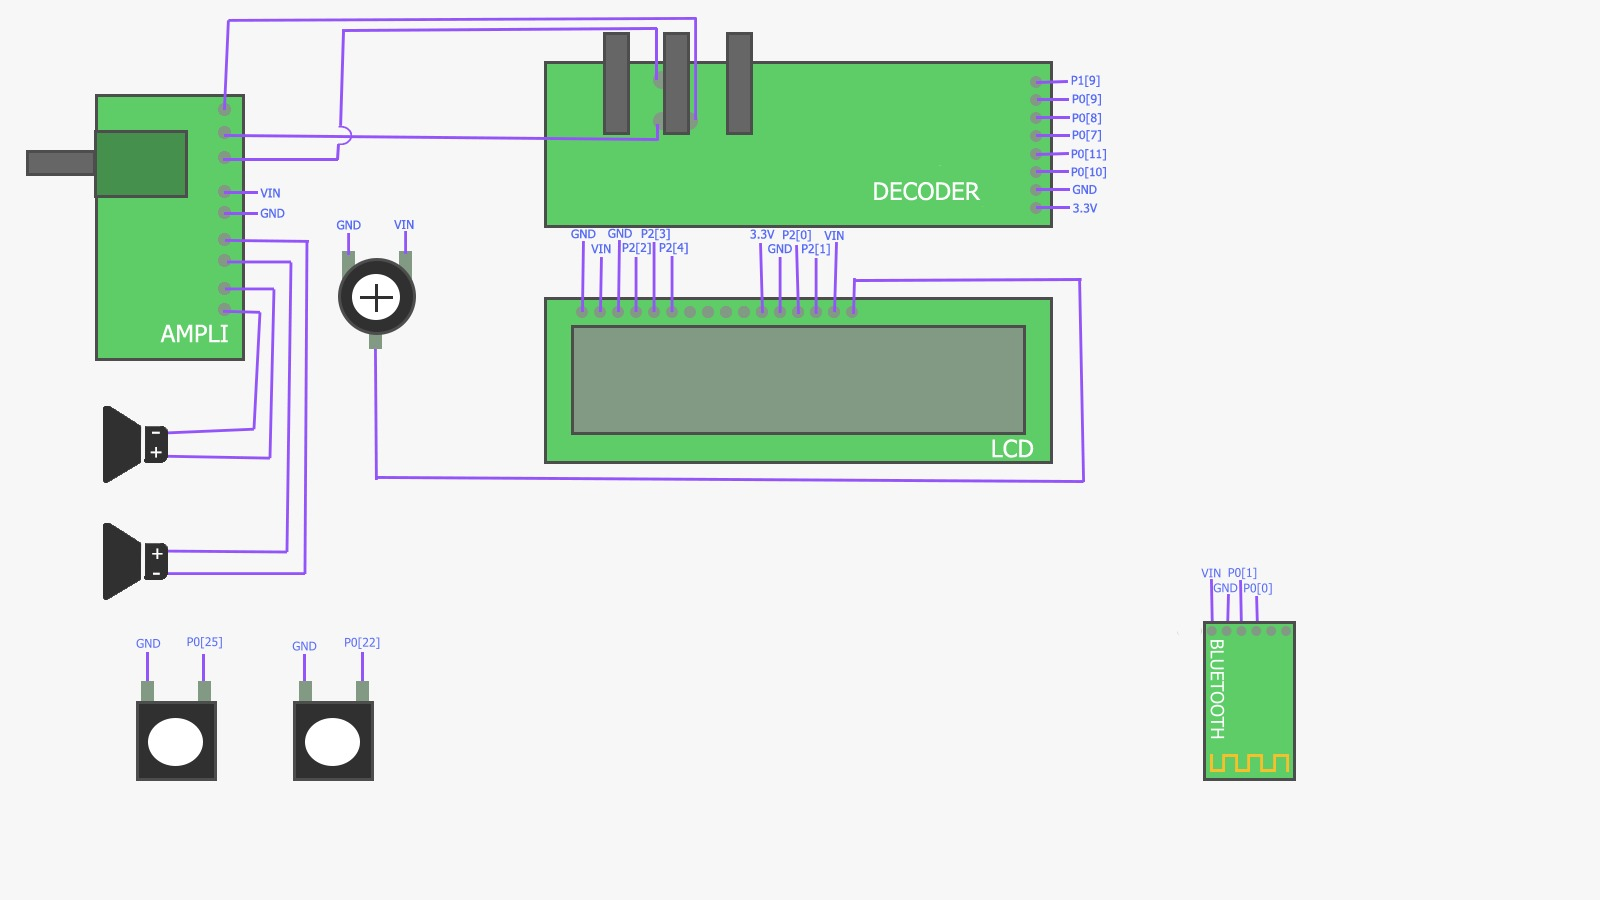
\includegraphics[scale=0.35]{Mapa.jpeg}
\end{center}


\chapter{Incidencias encontradas}
\section{Incidencias hardware}
A la hora de truncar los bits con un encoder, observamos que no funcionaba de forma correcta debido al mal estado del mismo. Como solución optamos por reemplazarlo por otro y al ver que no funciona tras varias pruebas e intentos, nos decidimos por poner dos pulsadores. Estos pulsadores tendrán la función de aumentar o decrementar los bits de resolución que tiene la canción (uno a uno) y que serán enviados al amplificador y luego a los altavoces.

Mediante las pruebas, tuvimos problemas con la antena bluetooth y lo solventamos usando una conexión por cable directa al puerto de entrada donde se conecta la antena bluetooth para no perder tiempo entre las pruebas esperando a que la antena bluetooth se conectara al portátil.

\section{Incidencias software}
A la hora de comenzar la canción, ésta no se oye correctamente debido a una estática presente en la muestra debido al buffer de entrada. La única solución encontrada es hacer un ``reset'' al dispositivo.

La interrupción EINT0 no es compatible con el encoder ya que daba lugar a varias activaciones de la misma sin que éste hubiera llamado a dicha interrupción. La solución ha sido cambiar la interrupción EINT0 por una interrupción de propósito general.


\chapter{Resultado final}
Finalmente hemos obtenido un altavoz bluetooth que tiene la peculiaridad de poder jugar con los bits de resolución de las canciones que se envían a través de CoolTerm\footnote{Es una aplicación que permite tener una terminal para nuestros puertos serie y desde su menú podemos elegir los puertos disponibles y seleccionar su velocidad y demás parámetros como el XON que lo usaremos en el envío de las muestras a la placa.} en un portátil.

También contamos con una pantalla que nos muestra el título de la canción que está sonando y los bits de resolución con los que se está escuchando la muestra.

Mientras más bits le vamos quitando podemos observar que va creciendo una estática en el audio, esto es debido a que los bits enviados a los altavoces son '0'.

Sin embargo, mediante el uso del dispositivo, podemos observar que repentinamente se para o la resolución con la que se escucha no es la adecuada e incluso podemos oír varios cambios de sonido y ``petardeos'' que nos sabemos a que son debidos.
	
\end{document}
